%
% Documento: Fundamentação Teórica
%

\chapter{Fundamentação Teórica}
\label{chap:fundamentacaoTeorica}

Para entendermos o porquê de utilizar mais de um banco de dados, temos que entender o que é um banco de dados, quais gêneros existem e para que tipo de problema cada gênero se destaca.


\section{Banco de Dados}
\label{sec:database}

Banco de dados é um sistema computadorizado de manutenção de registros \cite{CJDate}. Elmasri \cite{Elmasri} acredita que o uso do computador tem aumentado significativamente por causa dos bancos de dados e ainda afirma, que eles representam um papel crucial em quase todas as áreas que envolve computação.

Devido a essa importância da persistência dos dados Elmasri apresenta as principais características de uma abordagem que utiliza processamento de arquivos \textit{versus} a abordagem que utiliza o banco de dados. Essas características são: natureza autodescritiva do sistema de banco de dados, isolamento entre os programas e dados e abstração de dados, suporte para as múltiplas visões de dados e por fim compartilhamento de dados e processamento de transações de multiusuários.

Elmasri compara a natureza autodescritiva das duas abordagens afirmando que ao utilizar a abordagem do banco de dados é possível identificar a estrutura dos arquivos, formato e tipo de dados apenas acessando o catálogo do banco de dados. Já na abordagem utilizando o processamento tradicional dos arquivos essas definições de estrutura estarão no próprio programa da aplicação. Então esses dados poderão ser acessados apenas por esse programa, dificultando que um programa em outra linguagem leia, ou escreva esses dados.

Elmasri não cita a existência de bancos de dados sem catálogo, chamados de \textit{schemaless}. Apesar de não ter a declaração do tipo de estruturas de dados contidas no banco, os bancos de dados \textit{schemaless} faz a abstração dos dados da mesma maneira que os bancos de dados tradicionais.

Como identificado por Elsmari a abastração de dados não é feito no processamento tradicional de arquivos. Suponha que tenhamos diversos programas utilizando o mesmo arquivo para armazenar um tipo de dado. Se um desses programas precisar de acrescentar algum campo novo, todos os outros programas que acessam esse arquivo devem modificados para contemplar o no campo adicionado.
Já quando utilizamos a abordagem de banco de dados, a alteração da estrutura dos dados pode não influenciar no funcionamento dos outros programas.

Em relação a característica, suporte para múltiplas visões dos dados, Elsmari afirma que quando é utilizado o banco de dados, é possível ter diferentes visões sobre os dados, fazendo o cruzamento das informações. Com a abordagem de processamento de arquivo tradicional isso não é usual.


A última característica comparada por Elmasri é o compartilhamento de dados e o processamento de transação multiusuários, essa característica é essencial para que várias aplicações possam acessar e alterar os dados. Porém o sistema de gerenciamento do banco de dados deve ter implementado um controle de concorrência para garantir a atomicidade das transações.

Como revelado acima a utilização do banco de dados, facilita o desenvolvimento das aplicações, faz a abstração entre aplicação e dados e além disso faz o controle de concorrência.

\section{Figuras}
\label{sec:figuras}

Abaixo é apresentado um exemplo de figura.
A \autoref{fig:kdtree} aparece automaticamente na lista de figuras.
Para uso avançado de imagens no LATEX, recomenda-se a consulta de literatura especializada \cite{Goossens2007}.

\begin{figure}[!htb]
    \centering
    \caption{Exemplo da estrutura de uma árvore KD}
    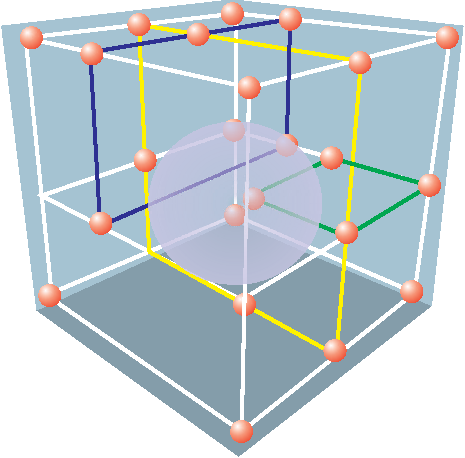
\includegraphics[width=0.3\textwidth]{./04-figuras/figkdtree}
    \fonte{\citeonline{CELSO2012}}
    \label{fig:kdtree}
\end{figure}

\section{Quadros e Tabelas}
\label{sec:tabelas}

Também é apresentado o exemplo do \autoref{qua:comparabd} e da \autoref{tab:correlacao}, que aparece automaticamente na lista de quadros e tabelas.
Informações sobre a construção de tabelas no LATEX podem ser encontradas na literatura especializada \cite{Lamport1986,Buerger1989,Kopka2003,Mittelbach2004}.

\begin{quadro}[!htb]
    \centering
    \caption{Hierarquia de restrições das questões.\label{qua:comparabd}}
    \begin{tabular}{|p{7cm}|p{7cm}|}
        \hline
        \textbf{BD Relacionais} & \textbf{BD Orientados a Objetos} \\
        \hline
        Os dados são passivos, ou seja, certas operações limitadas podem ser automaticamente acionadas quando os dados são usados. Os dados são ativos, ou seja, as solicitações fazem com que os objetos executem seus métodos. & Os processos que usam dados mudam constantemente. \\
        \hline
    \end{tabular}
    \fonte{\citeonline{carvalho:2001}}
\end{quadro}


Muitos confundem, mas existe diferença entre tabelas e quadros.
Um quadro é formado por linhas horizontais e verticais,
sendo, portanto ``fechado''. Normalmente é usado
para apresentar dados secundários. Nada impede, porém,
que um quadro apresente resultados da pesquisa.
Um quadro normalmente apresenta resultados
qualitativos (textos). O número do quadro e o título
vêm acima do quadro, e a fonte, deve vir abaixo.
Uma tabela é formada apenas por linhas verticais, sendo,
portanto ``aberta''. Normalmente é usada para
apresentar dados primários, e geralmente vem nos
``resultados'' e na discussão do trabalho. Nada
impede, porém, que uma tabela seja usada no
referencial teórico de um trabalho. Uma tabela
normalmente apresenta resultados quantitativos
(números). O número da tabela e o título vêm
acima da tabela, e a fonte, deve vir abaixo, como
no quadro.

Exemplos de tabelas:

\begin{table}[!htb]
    \centering
    \caption[Correlação de valores x e y]{Exemplo de uma tabela mostrando a correlação entre x e y.\label{tab:correlacao}}
    \begin{tabular}{cc}
        \hline
            x & y \\
        \hline
            1 & 2 \\
            3 & 4 \\
            5 & 6 \\
            7 & 8 \\
        \hline
    \end{tabular}
    \fonte{Autoria própria.}
\end{table}


\begin{table}[!htb]
    \centering
    \caption[Resultado dos testes]{Resultado dos testes.\label{tab:testes}}
    \begin{tabular}{rrrrr}
        \toprule
            & Valores 1 & Valores 2 & Valores 3 & Valores 4 \\
        \midrule
            Caso 1 & 0,86 & 0,77 & 0,81 & 163 \\
            Caso 2 & 0,19 & 0,74 & 0,25 & 180 \\
            Caso 3 & 1,00 & 1,00 & 1,00 & 170 \\
        \bottomrule
    \end{tabular}
\end{table}


\section{Equações}
\label{sec:equacoes}

A transformada de Laplace é dada na \autoref{eq:laplace}, enquanto a \autoref{eq:dft} apresenta a formulação da transformada discreta de Fourier bidimensional\footnote{Deve-se reparar na formatação esteticamente perfeita destas equações.}.

\begin{equation}
    X(s) = \int\limits_{t = -\infty}^{\infty} x(t) \, \text{e}^{-st} \, dt
    \label{eq:laplace}
\end{equation}

\begin{equation}
    F(u, v) = \sum_{m = 0}^{M - 1} \sum_{n = 0}^{N - 1} f(m, n) \exp \left[ -j 2 \pi \left( \frac{u m}{M} + \frac{v n}{N} \right) \right]
    \label{eq:dft}
\end{equation}

\section{Algoritmos}\label{sec:algoritmos}

Os algoritmos devem ser feitos segundo o modelo abaixo.
Para isso, utilizar o pacote {\ttfamily algorithm2e} no início do arquivo principal como neste exemplo.
O \autoref{alg:vertices} mostra um exemplo.

\begin{algorithm}
    \caption{Algoritmo para remoção aleatória de vértices}\label{alg:vertices}
    \KwIn{o número $n$ de vértices a remover, grafo original $G(V, E)$}
    \KwOut{grafo reduzido $G'(V,E)$}
    $removidos \leftarrow 0$ \\
    \While {removidos $<$ n } {
        $v \leftarrow$ Random$(1, ..., k) \in V$ \\
            \For {$u \in adjacentes(v)$} {
                remove aresta (u, v)\\
                $removidos \leftarrow removidos + 1$\\
            }
            \If {há  componentes desconectados} {
                remove os componentes desconectados\\
            }
        }
\end{algorithm}





